\documentclass[11pt,a4paper,bibliography=totocnumbered,listof=totocnumbered]{scrartcl}
\usepackage[ngerman]{babel}
\usepackage[utf8]{inputenc}
\usepackage{amsmath}
\usepackage{amsfonts}
\usepackage{amssymb}
\usepackage{graphicx}
\usepackage{fancyhdr}
\usepackage{tabularx}
\usepackage{geometry}
\usepackage{setspace}
\usepackage[right]{eurosym}
\usepackage[printonlyused]{acronym}
\usepackage{subfig}
\usepackage{floatflt}
\usepackage[usenames,dvipsnames]{color}
\usepackage{colortbl}
\usepackage{paralist}
\usepackage{array}
\usepackage{titlesec}
\usepackage{parskip}
\usepackage{url}
%\usepackage{picins}
\usepackage[subfigure,titles]{tocloft}
\usepackage[pdfpagelabels=true]{hyperref}
%\usepackage[dvipsnames]{xcolor}
\usepackage{courier} %für Inline Code
\usepackage[htt]{hyphenat} % ermöglicht Zeilenumbrüche bei Typewriterschriften 

\usepackage{booktabs} % schönere Tabellenlinien
\usepackage[table,xcdraw]{xcolor} %Für farbige Tabelle


\usepackage{listings}
\lstset{language=XML, 
	basicstyle=\scriptsize\sffamily, 
	keywordstyle=\color{RedViolet}\sffamily, 
	identifierstyle=, 
	captionpos=b,
	commentstyle=\color{OliveGreen}, 
	stringstyle=\sffamily, 
	breaklines=true, 
	%numbers=right, 
	%numberstyle=\small, 
	frame=single, 
	stringstyle=\ttfamily, 
%	frame = lrbt,
%	numbers = left,
	showstringspaces = false,
	breaklines = true,
%	xleftmargin = 30pt,
%	xrightmargin = 30pt,
}
	 
	 
	 
\makeatletter
\def\l@lstlisting#1#2{\@dottedtocline{1}{0em}{1em}{\hspace{1,5em} Lst. #1}{#2}}
\makeatother



\geometry{a4paper, top=27mm, left=25mm, right=25mm, bottom=35mm, headsep=10mm, footskip=12mm}

\hypersetup{unicode=false, pdftoolbar=true, pdfmenubar=true, pdffitwindow=false, pdfstartview={FitH},
	pdftitle={Facharbeit},
	pdfauthor={Hendrik Hofmann},
	pdfsubject={Abschlussarbeit},
	pdfcreator={\LaTeX\ with package \flqq hyperref\frqq},
	pdfproducer={pdfTeX \the\pdftexversion.\pdftexrevision},
	pdfkeywords={Abschlussarbeit},
	pdfnewwindow=true,
	colorlinks=true,linkcolor=black,citecolor=black,filecolor=magenta,urlcolor=black}


\begin{document}

\titlespacing{\section}{0pt}{12pt plus 4pt minus 2pt}{-6pt plus 2pt minus 2pt}

% Kopf- und Fusszeile
\renewcommand{\sectionmark}[1]{\markright{#1}}
\renewcommand{\leftmark}{\rightmark}
\pagestyle{fancy}
\lhead{}
\chead{}
\rhead{\thesection\space\contentsname}
\lfoot{}
\cfoot{}
\rfoot{\ \linebreak Seite \thepage}
\renewcommand{\headrulewidth}{1.0pt}
\renewcommand{\footrulewidth}{1.0pt}

% Vorspann
\renewcommand{\thesection}{\Roman{section}}
\renewcommand{\theHsection}{\Roman{section}}
\pagenumbering{Roman}

% ----------------------------------------------------------------------------------------------------------
% Titelseite
% ----------------------------------------------------------------------------------------------------------
\thispagestyle{empty}
\begin{center}
		\vspace*{.2cm}
		\begin{flushright}
			\advance\rightskip+2cm
			
\includegraphics[width=.4\textwidth]{img/HTW-quer-rgb.pdf} %\\[10cm]
		\end{flushright}
	\vspace*{3cm}
	\Large
	\textbf{Fachbereich IV}\\
	\textbf{Angewandte Informatik}\\
	\vspace*{2cm}
	{\rule{\linewidth}{0.5mm}}
	\Huge
	\textbf{Hausarbeit}\\
	\vspace*{0.5cm}
	\large
	über das Thema\\
	\vspace*{1cm}
	\textbf{Versuch einer \textit{'lege artis' Analyse} der Software Device Registration}\\
	{\rule{\linewidth}{0.5mm}}
	\vspace*{2cm}
	
	\vfill
	\normalsize
		\begin{minipage}[t]{0.4\textwidth}
			\begin{flushleft} %\large
				%\emph{Author:}\\
				
				Hendrik Hofmann\\ Matr.Nr.: 539721 \\7.Semester \\{\today}
				
			\end{flushleft}
		\end{minipage}
		\begin{minipage}[t]{0.3\textwidth}
			\begin{flushright} %\large
				  Prüfer: \\Prof. Dr.-Ing. habil. \\Dierk Langbein, \\ Onur Yavuz
			\end{flushright}
		\end{minipage}
\end{center}
\pagebreak



% ----------------------------------------------------------------------------------------------------------
% Verzeichnisse
% ----------------------------------------------------------------------------------------------------------
% TODO Typ vor Nummer
\renewcommand{\cfttabpresnum}{Tab. }
\renewcommand{\cftfigpresnum}{Abb. }
\settowidth{\cfttabnumwidth}{Abb. 10\quad}
\settowidth{\cftfignumwidth}{Abb. 10\quad}

\titlespacing{\section}{0pt}{12pt plus 4pt minus 2pt}{2pt plus 2pt minus 2pt}
\singlespacing
\rhead{INHALTSVERZEICHNIS}
\renewcommand{\contentsname}{I Inhaltsverzeichnis}
\phantomsection

\addtocounter{section}{1}
\tableofcontents
\pagebreak

\pagebreak

%\pagebreak


\pagebreak



% ----------------------------------------------------------------------------------------------------------
% Inhalt
% ----------------------------------------------------------------------------------------------------------
% Abstände Überschrift
%\titlespacing{\section}{10pt}{12pt plus 4pt minus 2pt}{-6pt plus 2pt minus 2pt}
%\titlespacing{\subsection}{10pt}{12pt plus 4pt minus 2pt}{-6pt plus 2pt minus 2pt}
%\titlespacing{\subsubsection}{10pt}{12pt plus 4pt minus 2pt}{-6pt plus 2pt minus 2pt}

% Kopfzeile
\renewcommand{\sectionmark}[1]{\markright{#1}}
\renewcommand{\subsectionmark}[1]{}
\renewcommand{\subsubsectionmark}[1]{}
\lhead{}
\rhead{\rightmark}

\onehalfspacing


\renewcommand{\thesection}{\arabic{section}}
\renewcommand{\theHsection}{\arabic{section}}
\setcounter{section}{0}
\pagenumbering{arabic}
\setcounter{page}{1}

% ----------------------------------------------------------------------------------------------------------
% Hier wird der eigentliche Text eingefügt
% ----------------------------------------------------------------------------------------------------------
\section{Grundlagen}
	\subsection{Der BMECat}
	
	Der BMECat ist ein vom 'Bundesverband Materialwirtschaft, Einkauf und Logistik e.V' in Zusammenarbeit mit dem 'eBusiness Standardization Committee' entwickelter XML
	Standard mit dem Ziel den Austausch von Produktkatalogen zwischen Lieferanten und beschaffenden Organisationen zu standardisieren und somit zu vereinfachen.\footnote{BMECat V1.2 Spezifikation, Seite 5}. 
	
	\subsubsection{Terminologie}
	Ein \textbf{Produktkatalog} ist die Menge aller benötigten Daten, welche vom katalogerzeugenden Unternehmen an das katalogempfangende Unternehmen übermittelt werden sollen.\\
	Ein \textbf{Katalogdokument} ist eine XML-Datei, in der der Produktkatalog im BMECat-Format gespeichert und zum Katalogemfänger übermittelt wird.\\
	Eine \textbf{Kataloggruppe} ist ein Datenbereich, der eine Gruppe definiert, welcher gleichartige Artikel zugeordnet werden können. Diese wird im BMEcat-Format durch das Element \texttt{\textbf{CATALOG\_STRUCTURE}} abgebildet.\\
	Ein \textbf{Kataloggruppensystem} ist ein hierarchischer Baum von verknüpften Kataloggruppen. Es wird
	im BMEcat-Format durch das Element \texttt{\textbf{CATALOG\_GROUP\_SYSTEM}} abgebildet.\footnote{BMECat V1.2 Spezifikation, Seite 7}
	
	\subsubsection{Transaktionen}
	Im BMECat wird zwischen den 3 verschiedenen Transaktionsarten
	\begin{itemize}
	\item \texttt{\textbf{T\_NEW\_CATALOG}} - Übertragung eines neuen Produktkataloges
	\item \texttt{\textbf{T\_UPDATE\_PRODUCTS}} - Aktualisierung von Produktdaten
	\item \texttt{\textbf{T\_UPDATE\_PRICES}} - Aktualisierung von Preisinformationen
	\end{itemize} 
	unterschieden. Die Unterscheidung geschieht um die Größe eines Katalogdokumentes zu reduzieren. Es muss so z.B. nicht ein kompletter Produktkatalog übertragen werden, falls sich bei einem \(oder mehreren\) Artikel\(n\) der Preis ändert.
	
	\subsubsection{Aufbau}
	
	Ein BMECat-Dokument besteht aus einer Folge von KANN und MUSS Feldern, den dazugehörigen Datentypen und Feldlängen und ist folgendermaßen aufgebaut:
		
		\begin{enumerate}
		
			\item XML-Deklaration und Header-Bereich (mit Informationen über Kataloganbieter und Empfänger, Bezeichnung und Erstellungsdatum des Kataloges etc.  )
				\\Bsp. für einen Header:
			\begin{lstlisting}
			<HEADER>
			  <GENERATOR_INFO> Kann </GENERATOR_INFO>
			  <CATALOG> Muss </CATALOG>
			  <BUYER> Kann </BUYER>
			  <SUPPLIER> Muss </SUPPLIER>
			</HEADER>
			\end{lstlisting}
			Bsp. für XML Deklaration:
			\begin{lstlisting}
			<?xml version="1.0" encoding="UTF-8"?>
			<!DOCTYPE BMECAT SYSTEM "bmecat_new_catalog.dtd">
			<BMECAT version="1.2" xml:lang="de" xmlns="http://www.bmecat.org/bmecat/1.2/bmecat_new_catalog">
			\end{lstlisting}
			\item Produktgruppensystem (Baumstruktur der Produktgruppen mit den Attributwerten Root, Node und Leaf)
			\begin{lstlisting}
			<CATALOG_STRUCTURE type="root">
			   <GROUP_ID>1</GROUP_ID>
			   <GROUP_NAME>Katalog</GROUP_NAME>
			   <PARENT_ID>0</PARENT_ID>
			   <GROUP_ORDER>1</GROUP_ORDER>
			</CATALOG_STRUCTURE>
			  <CATALOG_STRUCTURE type="node">
			   <GROUP_ID>2</GROUP_ID>
			   <GROUP_NAME>Spiele &amp; Konsolen</GROUP_NAME>
			   <PARENT_ID>1</PARENT_ID>
			 </CATALOG_STRUCTURE>
			 <CATALOG_STRUCTURE type="leaf">
			   <GROUP_ID>7</GROUP_ID>
			   <GROUP_NAME>PlayStation 4</GROUP_NAME>
			   <PARENT_ID>2</PARENT_ID>
			 </CATALOG_STRUCTURE>
			\end{lstlisting}
			
			
			
			\item Artikel (mit Attributen und Werten)
			
			\begin{lstlisting}
			<ARTICLE mode="new">
				<SUPPLIER_AID>9057320097280</SUPPLIER_AID>
				<ARTICLE_DETAILS>
				   	<DESCRIPTION_SHORT>GTA 5</DESCRIPTION_SHORT>
					<DESCRIPTION_LONG>Das tolle neue Spiel</DESCRIPTION_LONG>
					<EAN>87126723434</EAN>
				... weitere Attribute ...
				</ARTICLE_DETAILS>
				...weitere Felder ...
			</ARTICLE>
			\end{lstlisting}
			
	
			\item Zuordnung der Artikel zu den Produktgruppen.
			\begin{lstlisting}
			<ARTICLE_TO_CATALOGGROUP_MAP>
				<ART_ID>9057320097280</ART_ID>
				<CATALOG_GROUP_ID>7</CATALOG_GROUP_ID>
			</ARTICLE_TO_CATALOGGROUP_MAP>
			\end{lstlisting}
		
		\end{enumerate}
		
	--- Übersicht der im BMECat verwendeten Datentypen --- noch einfügen ---
	
	Im folgenden Abschnitt wird jeder Teilbereich mit seinen Unterelementen, wie sie in vorliegender Arbeit verwandt wurden, graphisch dargestellt und kurz erläutert. Rot hervorgehoben sind jeweils die MUSS-Felder, welche zwingend in einem gültigen BMECat Dokument vorkommen müssen, grün die KANN-Felder. Ein Plus \(+\) Zeichen hinter dem Elementnamen indiziert, dass dieses Element mehrfach an dieser Stelle vorkommen kann, jedoch mindestens einmal. Ein Asterisk \(*\) zeigt an, dass dieses Element einmal, mehrfach oder nicht vorkommen kann. Das 
	
	\textbf{\underline{Header}}\\
	Im Header werden allgemeine Informationen über das Katalogdokument hinterlegt und Default Werte gesetzt. Das Element \texttt{\textbf{CATALOG}} enthält dabei Informationen zur Identifikation und Beschreibung des Produktkataloges, wie z.B. die Katalog Id, die Katalogversion oder die für das Dokument geltende Sprache sowie Elemente zum setzten von Standard-Werten wie z.B. die für das Katalogdokument geltende Währungsangabe \footnote{BMECat V 1.2 Spezifikation, Seite 27,29} 
	
	\begin{minipage}{\linewidth}
		\vspace{1em}
		\centering
		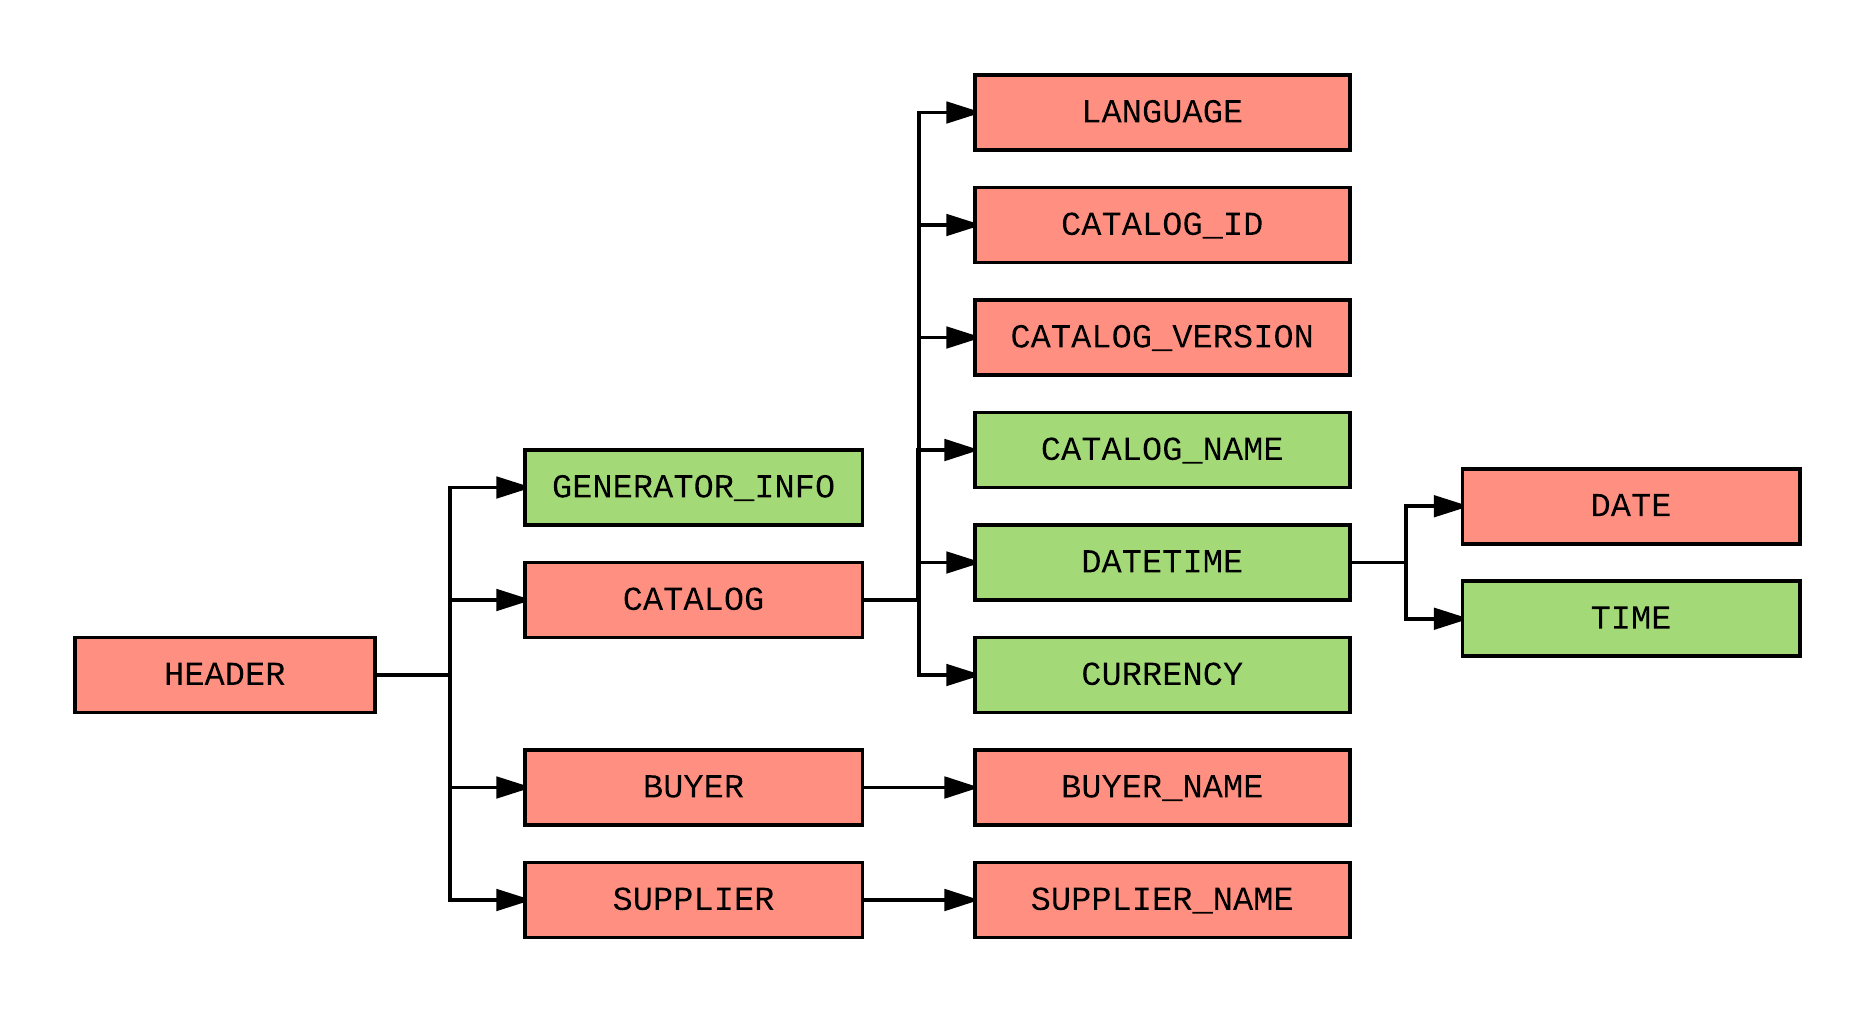
\includegraphics[width=1\linewidth]{img/BMECat_Header}
		\captionof{figure}[Headerstruktur]{Headerstruktur}
		\label{fig:header}
		\vspace{1em}
	\end{minipage}
	
	
	
	\textbf{\underline{Die Transaktion T\_NEW\_CATALOG}}
	
	Diese Transaktion wird verwandt, um einen Produktkatalog neu zu übertragen. Das empfangende System reagiert dabei je nach übertragener \texttt{CATALOG\_ID}, \texttt{CATALOG\_VERSION}
	und \texttt{LANGUAGE} unterschiedlich. Dieser Zusammenhang wir später noch erläutert.
	
	
	\begin{minipage}{\linewidth}
		\vspace{1em}
		\centering
		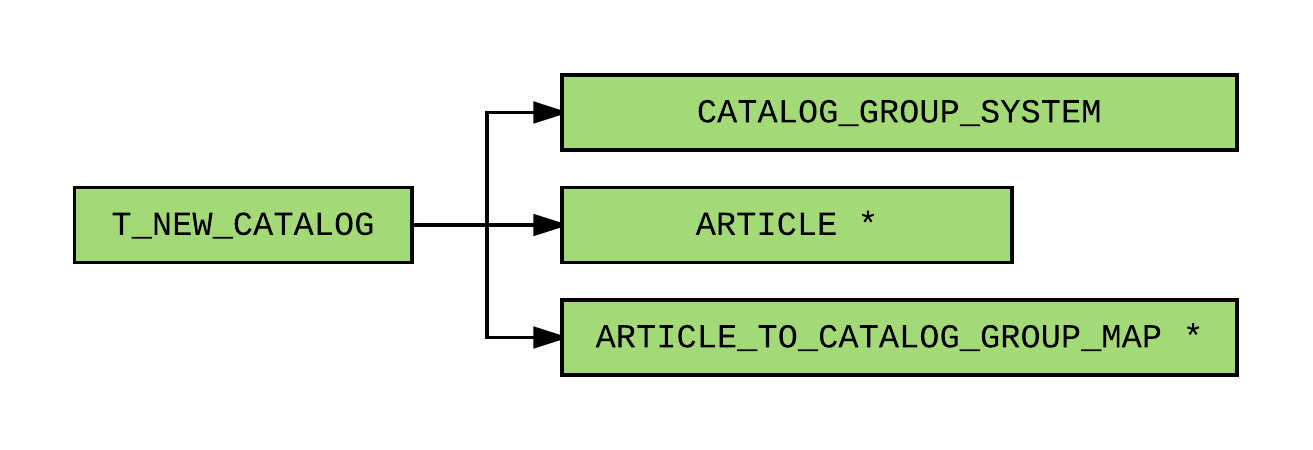
\includegraphics[width=0.8\linewidth]{img/newCatalog}
		\captionof{figure}[T\_NEW\_CATALOG]{T\_NEW\_CATALOG}
		\label{fig:header}
		\vspace{1em}
	\end{minipage}
	
	\textbf{\underline{Die Transaktion T\_UPDATE\_PRODUCTS}}\\
	
	Bei dieser Transaktion werden Artikeldaten übertragen und gegebenenfalls einer Kataloggruppe zugeordnet.Je nach Kennung des Artikels (s.u.)  werden die übertragenen
	Artikel im Zielsystem entweder hinzugefügt, gelöscht oder die Artikeldaten werden komplett ersetzt.
	Der Artikel wird immer komplett ausgetauscht, eine Änderung von einzelnen Datenfeldern innerhalb eines Artikels ist nicht möglich.
	Wie der Grafik entnommen werden kann ist bei dieser Transaktion nur die Übertragung von Produktdaten und die Zuordnung von Produkten zu Kataloggruppen möglich. \footnote{vgl. BMECat V 1.2 Spezifikation, Seite 52}
	
	\begin{minipage}{\linewidth}
		\vspace{1em}
		\centering
		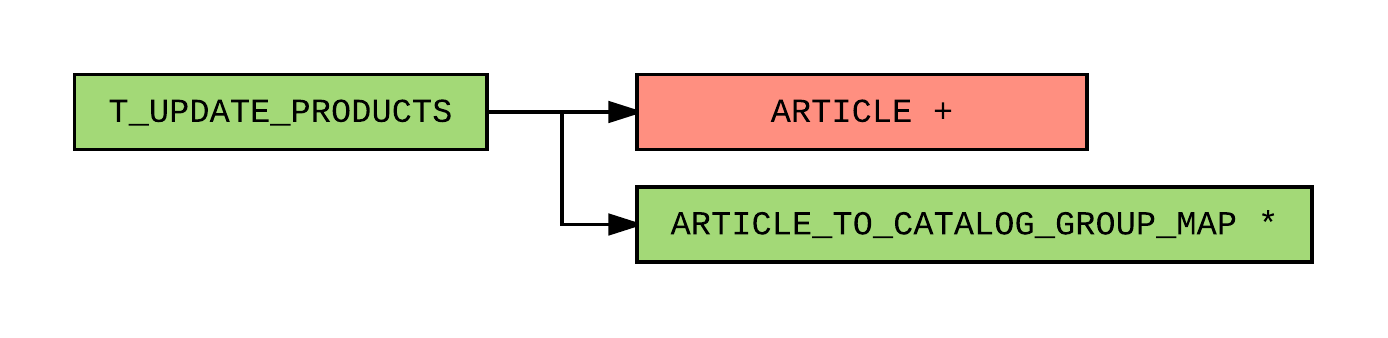
\includegraphics[width=0.8\linewidth]{img/updateProducts}
		\captionof{figure}[T\_UPDATE\_PRODUCTS]{T\_UPDATE\_PRODUCTS}
		\label{fig:header}
		\vspace{1em}
	\end{minipage}
	
	Das Element \texttt{T\_UPDATE\_PRODUCTS} verfügt zusätzlich über das Attribut \texttt{prev\_version}, welches die Anzahl der vorausgegangenen Updates bzw. die Nummer des übertragenen Updates enthält. 
	
	\begin{lstlisting}
	<T_UPDATE_PRODUCTS prev_version="91">...</T_UPDATE_PRODUCTS>
	\end{lstlisting}
	
	
	
	\textbf{\underline{Die Elemente CATALOG\_GROUP\_SYSTEM und CATALOG\_STRUCTURE}}\\
	
	Im Element \texttt{CATALOG\_GROUP\_SYSTEM} werden die \texttt{GROUP\_SYSTEM\_ID} und der \texttt{GROUP\_SYSTEM\_NAME} bekannt gemacht sowie die Katalogstruktur  \texttt{CATALOG\_STRUCTURE}   beschrieben. Dabei gibt es genau ein Wurzelelement, sowie beliebig viele Knoten und Blätter. Jedes Element hat dabei eine als \texttt{GROUP\_ID} bezeichnete ID und wird über \texttt{PARENT\_ID} die  dem jeweiligen Elternelement zugeordnet. Die Zuordnung der Artikel zu den Artikelgruppen erfolgt mit dem Element \texttt{ARTICLE\_TO\_CATALOG\_GROUP\_MAP} das weiter unten beschrieben wird.
	
	\begin{minipage}{\linewidth}
		\vspace{1em}
		\centering
		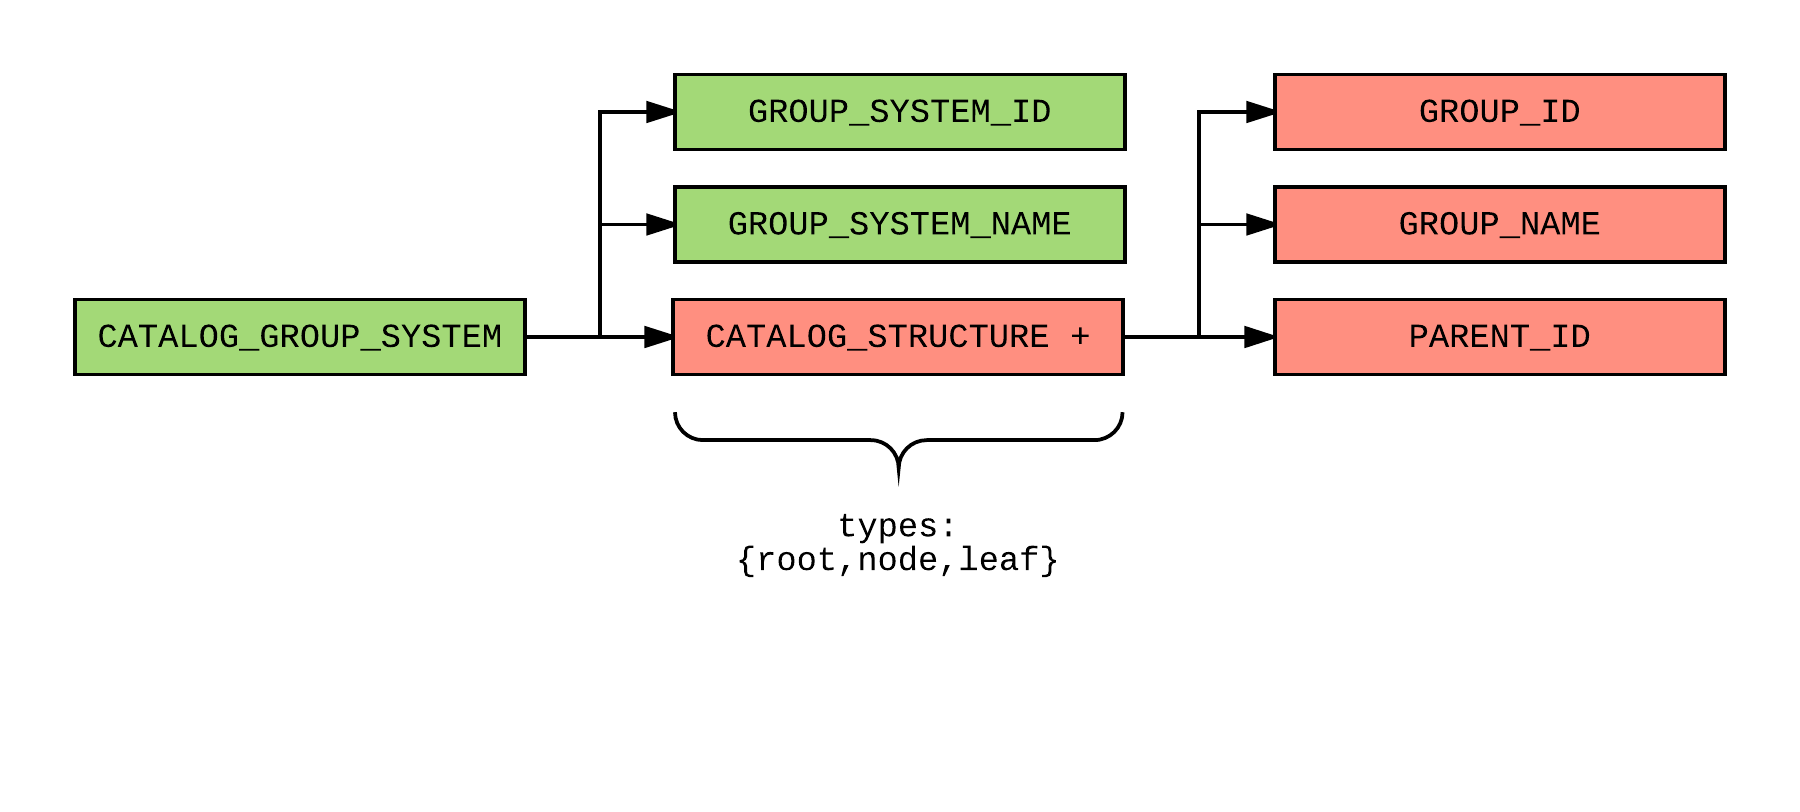
\includegraphics[width=0.7\linewidth]{img/catalogGroupSystem}
		\captionof{figure}[CATALOG\_GROUP\_SYSTEM und CATALOG\_STRUCTURE]{CATALOG\_GROUP\_SYSTEM und CATALOG\_STRUCTURE}
		\label{fig:header}
		\vspace{1em}
	\end{minipage} \pagebreak
	
	\textbf{\underline{Das Element ARTICLE}}\\
	Das Artikelelement schließlich enthält Informationen über einen Artikel, wie Überschrift, Beschreibung, Bilder, Preisinformationen, eine \textbf{eindeutige} Artikelnummer usw. Die Artikelnummer wird über das Element \texttt{SUPPLIER\_AID} bekanntgegeben, handelt es sich um einen Variantenartikel, so bildet sich die Artikelnummer aus der \texttt{SUPPLIER\_AID} und der \texttt{SUPPLIER\_AID\_SUPPLEMENT}. Dies ist hier jedoch nicht umgesetzt. Die als \textit{eCl@ass} und \textit{Zolltarifnummer} zusammengefassten \texttt{ARTICLE\_FEATURES} werden explizit von Mercateo verlangt.
	
	\begin{minipage}{\linewidth}
		\vspace{1em}
		\centering
		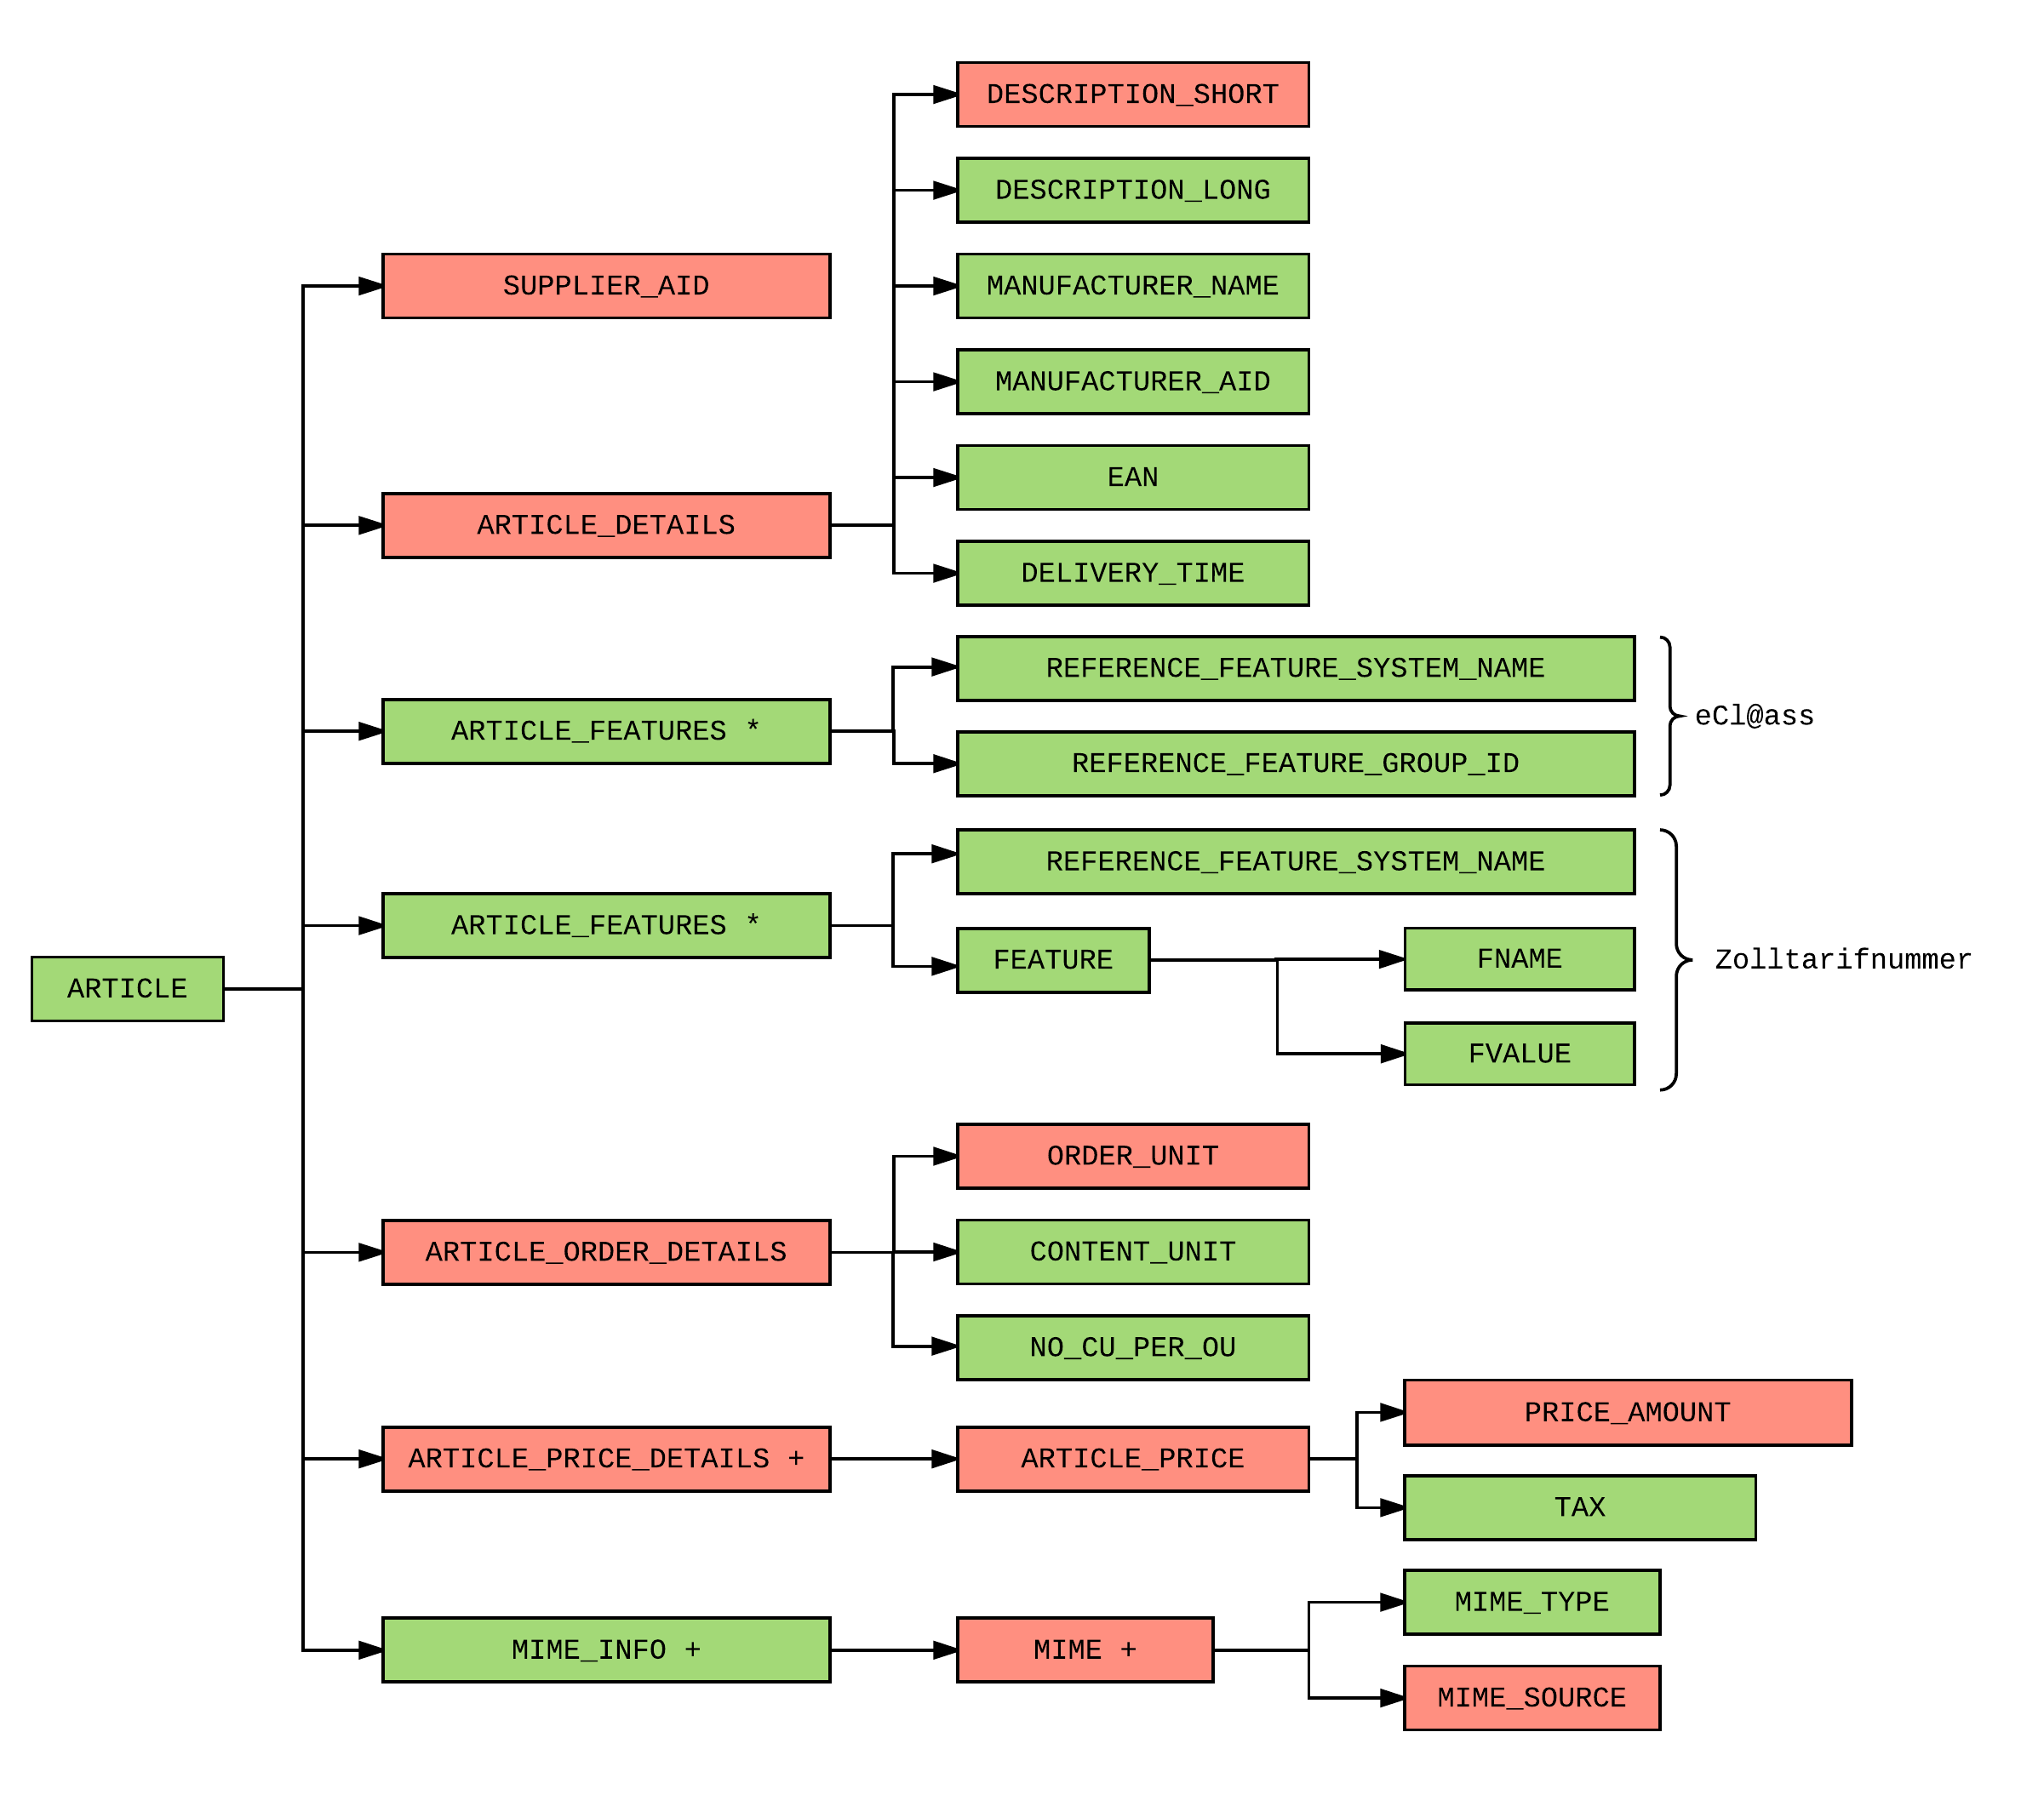
\includegraphics[width=1\linewidth]{img/Article}
		\captionof{figure}[Article]{Article}
		\label{fig:header}
		\vspace{1em}
	\end{minipage}
	
	Das Element \texttt{ARTICLE} verfügt über das Attribut \texttt{mode}, welches Informationen darüber enthält, ob es sich um die Anlage eines neuen Artikel, ein Update der Artikelinformationen oder die Löschung eines Artikels handelt.
	
	\begin{lstlisting}
	<ARTICLE mode="new">...</ARTICLE>
	<ARTICLE mode="update">...</ARTICLE>
	<ARTICLE mode="delete">...</ARTICLE>
	\end{lstlisting}
	
	
	
	\textbf{\underline{Das Element ARTICLE\_TO\_CATALOG\_GROUP\_MAP}}\\
	
	Um Produkte ihren Kategorien zuordnen zu können wird das Element \texttt{ARTICLE\_TO\_CATALOGGROUP\_MAP} verwandt. Es erfolgt hier eine Verknüfung aus der eindeutigen Artikelnummer und der \texttt{GROUP\_ID} welcher der Artikel zugeordnet werden soll. Eine Mehrfachzuordnung ist möglich, d.h. ein Artikel kann in unterschiedliche Kategorien "eingehängt" werden.
	
	\begin{minipage}{\linewidth}
		\vspace{1em}
		\centering
		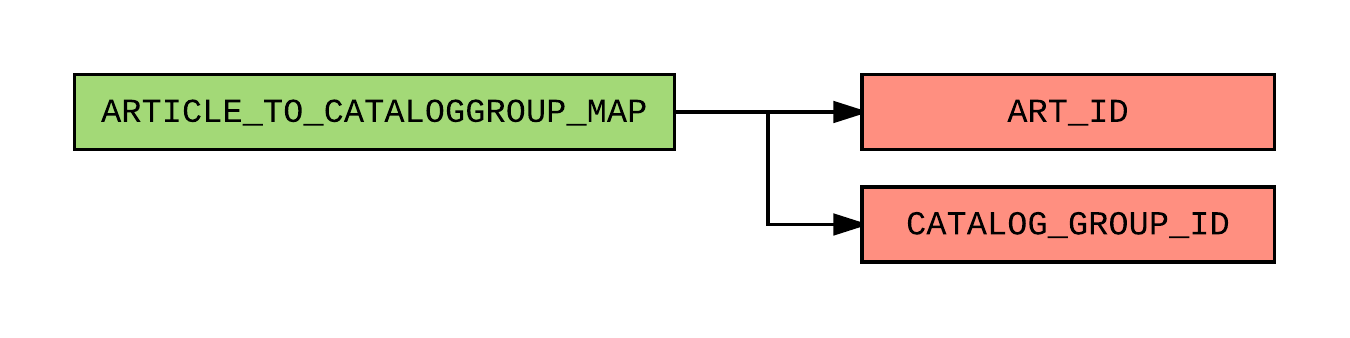
\includegraphics[width=0.7\linewidth]{img/articleGroupMap}
		\captionof{figure}[ArticleGroupMap]{ARTICLE\_TO\_CATALOG\_GROUP\_MAP}
		\label{fig:header}
		\vspace{1em}
	\end{minipage}
	
	Im Kontext der Transaktion \texttt{T\_UPDATE\_PRODUCTS} verfügt das Element zusätzlich über das Attribut \texttt{mode}, mit welchem angegeben wird, ob es sich um eine Neuzuweisung zu einer Kategorie handelt oder der Artikel aus einer Kategorie entfernt werden soll.
	
	\begin{lstlisting}
	<ARTICLE_TO_CATALOGGROUP_MAP mode="new">...</<ARTICLE_TO_CATALOGGROUP_MAP>
	<ARTICLE_TO_CATALOGGROUP_MAP mode="delete">...</<ARTICLE_TO_CATALOGGROUP_MAP>
	\end{lstlisting}
	
	
	\textbf{\underline{Zusammenspiel verschiedener Transaktionen}}\\
	
	Die folgende Grafik zeigt, wie das empfangende System bei der Transaktion \texttt{T\_NEW\_CATALOG} je nach übergebener \texttt{CATALOG\_ID}, \texttt{CATALOG\_VERSION} und \texttt{LANGUAGE} reagiert.
	
	\begin{minipage}{\linewidth}
		\vspace{1em}
		\centering
		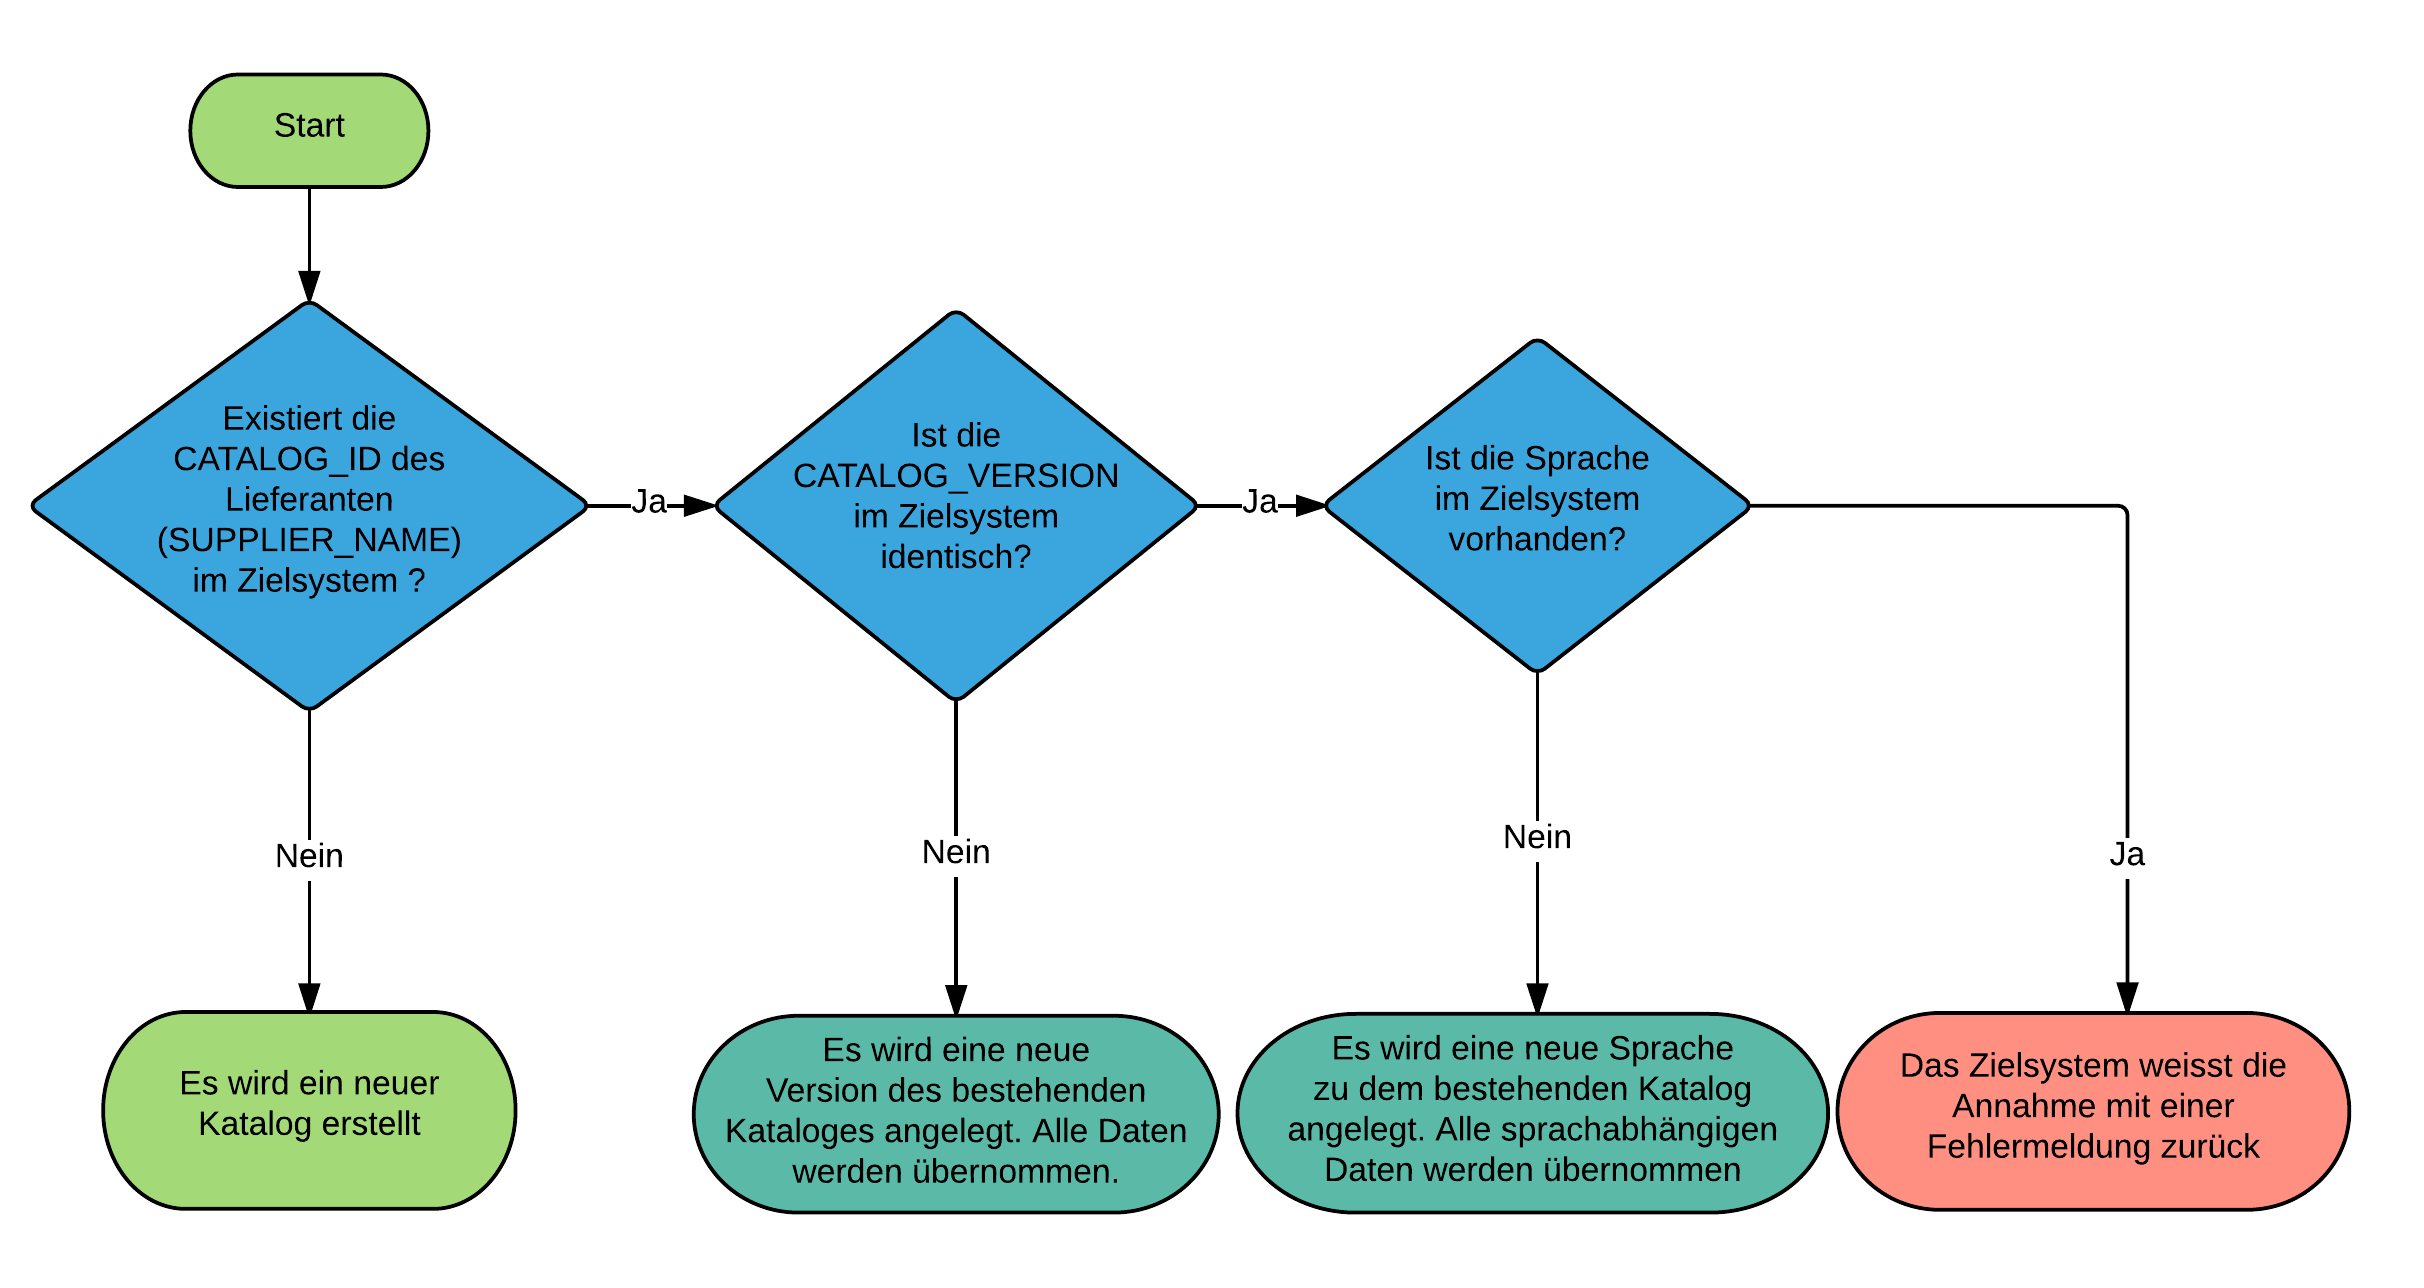
\includegraphics[width=1\linewidth]{img/newCatalogLogik}
		\captionof{figure}[New Catalog Logik]{Flowchart T\_NEW\_CATALOG}
		\label{fig:header}
		\vspace{1em}
	\end{minipage}
	
	Kommt die Transaktion \texttt{T\_UPDATE\_PRODUCTS} zur Anwendung, gilt es folgendes zu beachten:\footnote{vgl. hierzu BMECat V 1.2 Spezifikation, Seite 52} 
	\begin{itemize}
		\item Die übertragene \texttt{CATALOG\_ID} des jeweiligen Lieferanten und die dazugehörige\\ \texttt{CATALOG\_VERSION} müssen im Zielsystem bereits vorhanden sein.
		\item Das Attribut \texttt{prev\_version} muss bei der ersten anderen Transaktionsart nach\\ \texttt{T\_NEW\_CATALOG}, (\texttt{T\_UPDATE\_PRODUCTS},\texttt{T\_UPDATE\_PRICES}) auf '0' gesetzt werden.
		\item Danach wird es bei jeder solchen Transaktion um '1' erhöht.
	\end{itemize}
	
	\section{Analyse der Aufgabe und der Anforderungen}
	
	\subsection{Bewertung von theoretischen Ansätzen, Konzepten, Methoden, Verfahren}
		lorem ipsum trallalala
	
	\subsection{Informelle Aufgabenbeschreibung}
	Ziel der Arbeit ist es die von der Software iTool aus verwaltbaren, in verschiedenen Tabellen einer SQL-Datenbank gehaltenen Produkt-, Katalog- Kategorie- und Herstellerdaten in ein von Mercateo verarbeitbares Format (dem BMECat) zu bringen. Dabei gilt es, den Anforderderungen der Spezifikationen sowohl das BMECat, als auch der besonderen Anforderungen seitens Mercateo zu genügen.
	Es soll möglich sein, die erwähnten Daten aus dem UI des iTool heraus nach dem CRUD-Prinzip zu bearbeiten. 
	Die eigentliche Erstellung der unterschiedlichen Kataloge (neuer Katalog bzw. Produktupdatekatalog) erfolgt dabei (automatisiert) über die CakePHP Shell. Kataloge können dabei für unterschiedliche Verkäufer erstellt werden.
	Zudem soll es Meracteo ermöglicht werden Bestandsdaten zu einer bestimmten Artikelnummer über ein Webinterface abzurufen.
	
	\subsection{Zielstellung}
	
	Folgende Funktionalitäten sollen implementiert werden:
	
	\begin{itemize}
	\item Die in iTool hinterlegten Produkt- bzw. Herstellerdaten sollen in ein gültiges und vollständiges BMECat Dokument entsprechend der Mercateo Anfoderungen überführt werden. Dabei ist insbesondere auf die Unterschiede und Besonderheiten der notwendigen beiden Transaktionsarten "T\_NEW\_CATALOG" - also die Erstellung eines neuen Kataloges - und "T\_UPDATE\_PRODUCTS" - also der Änderungen von Produktdaten, sowie dem löschen und neu erstellen von Produkten - zu achten .
		\begin{itemize}
		\item Gültig bedeutet in diesem Fall, dass Struktur und Inhalt des Dokuments fehlerfrei gegen die entsprechende XSD Datei laufen, d.h. die Felder müssen in der richtigen Reihenfolge unter Beachtung der Datentypen und Längenbegrenzungen sowie Formatlimitierungen (z.B. keine Sonderzeichen in der SKU (o.ä.)) geschrieben werden.
		\item Vollständig heißt, dass zum einen mindestens jene Felder im BMECat Dokument vorkommen, die die BMECat Spezifikation verlangt.Zusätzlich müssen jene Felder vorkommen, die die Mercateo Spezifikation erfordert und zwar unter zusätzlicher Beachtung der Limitierungen bzw. Besonderheiten jener Spezifikation. 	
		\end{itemize}
		
	\item Die Produktkategoriestruktur des iTool soll in das Kataloggruppensystem des BMECat überführt werden.
	\item die Implementierung der Katalogerstellungslogik erfolgt in einer Cake Shell. Liegt noch kein Katalog vor, wird ein neuer Katalog erstellt; ein Updatekatalog wird erstellt, wenn es Änderungen bei den Produktdaten gab. 
	\item Kataloge können für unterschiedliche Verkäufer erstellt werden.
	\item Die Produkt und Katalogdaten können über die Benutzeroberfläche des iTool eingesehen bzw. verändert werden. 
	\item Es soll Mercateo ermöglicht werden Bestandsdaten zu den im Katalog vermerkten Produkten über ein Webinterface abzurufen.
	\item Bei der Katalogerstellung ist darauf zu achten, dass es zu keinen Arbeitsspeicherüberläufen kommen kann.
	\end{itemize}
	

	
	





% ----------------------------------------------------------------------------------------------------------
% Kapitel
% ----------------------------------------------------------------------------------------------------------

% Bilder anzeigen

%\listfigurename





% ----------------------------------------------------------------------------------------------------------
% Literatur
% ----------------------------------------------------------------------------------------------------------
\renewcommand\refname{Quellenverzeichnis}
\bibliographystyle{myalpha}
\bibliography{bibo}
\vspace{10px}
\begin{enumerate}
	
	\item Fowler, Martin ; Beck, Kent ; Brant, John ; Opdyke, William ; Roberts, Don ; Gamma, Erich: Refactoring : Improving the Design of Existing Code. 1. Aufl.. Amsterdam: Addison-Wesley, 2012.
	\item Martin, Robert C.: Clean Code - Refactoring, Patterns, Testen und Techniken für sauberen Code : Deutsche Ausgabe. 1. Aufl.. Heidelberg: MITP-Verlags GmbH \& Co. KG, 2013.
	\item Hauer, Phillip ; philliphauer.de; http://www.philipphauer.de/study/se/design-pattern.php; Abgerufen am 29.3.2016;
\end{enumerate}


\pagebreak

% ----------------------------------------------------------------------------------------------------------
% Anhang
% ----------------------------------------------------------------------------------------------------------


\end{document}
